\documentclass{uai2023} % for initial submission
% \documentclass[accepted]{uai2023} % after acceptance, for a revised
                                    % version; also before submission to
                                    % see how the non-anonymous paper
                                    % would look like

%% There is a class option to choose the math font
% \documentclass[mathfont=ptmx]{uai2023} % ptmx math instead of Computer
% Modern (has noticable issues)
% \documentclass[mathfont=newtx]{uai2023} % newtx fonts (improves upon
 % ptmx; less tested, no support)
% NOTE: Only keep *one* line above as appropriate, as it will be replaced
%       automatically for papers to be published. Do not make any other
%       change above this note for an accepted version.

%% Choose your variant of English; be consistent
\usepackage[american]{babel}
% \usepackage[british]{babel}

%% Some suggested packages, as needed:
\usepackage{natbib} % has a nice set of citation styles and commands
    \bibliographystyle{plainnat}
    \renewcommand{\bibsection}{\subsubsection*{References}}
\usepackage{mathtools} % amsmath with fixes and additions
% \usepackage{siunitx} % for proper typesetting of numbers and units
\usepackage{booktabs} % commands to create good-looking tables
\usepackage{tikz} % nice language for creating drawings and diagrams

% for cross referencing the main text
% PLEASE ONLY USE xr IN THE SUPPLEMENTARY MATERIAL. 
% In the main paper, hard code any cross-reference to the supplementary material. 
\usepackage{xr}

%% Copied from https://www.overleaf.com/learn/how-to/Cross_referencing_with_the_xr_package_in_Overleaf#When_should_I_use_the_xr_package.3F
\makeatletter
\newcommand*{\addFileDependency}[1]{% argument=file name and extension
\typeout{(#1)}% latexmk will find this if $recorder=0
% however, in that case, it will ignore #1 if it is a .aux or 
% .pdf file etc and it exists! If it doesn't exist, it will appear 
% in the list of dependents regardless)
%
% Write the following if you want it to appear in \listfiles 
% --- although not really necessary and latexmk doesn't use this
%
\@addtofilelist{#1}
%
% latexmk will find this message if #1 doesn't exist (yet)
\IfFileExists{#1}{}{\typeout{No file #1.}}
}\makeatother

\newcommand*{\myexternaldocument}[2][]{%
\externaldocument[#1]{#2}%
\addFileDependency{#2.tex}%
\addFileDependency{#2.aux}%
}
%------------End of helper code--------------

% put all the external documents here!
\myexternaldocument[main-]{main}

%% Provided macros
% \smaller: Because the class footnote size is essentially LaTeX's \small,
%           redefining \footnotesize, we provide the original \footnotesize
%           using this macro.
%           (Use only sparingly, e.g., in drawings, as it is quite small.)

%% Self-defined macros
\newcommand{\swap}[3][-]{#3#1#2} % just an example

\title{Fast and Scalable Score-Based Calibration Tests\\(Supplementary Material)}

% The standard author block has changed for UAI 2023 to provide
% more space for long author lists and allow for complex affiliations
%
% All author information is authomatically removed by the class for the
% anonymous submission version of your paper, so you can already add your
% information below.
%
% Add authors
\author[1]{\href{mailto:<jj@example.edu>?Subject=Your UAI 2023 paper}{Jane~J.~von~O'L\'opez}{}}
\author[1]{Harry~Q.~Bovik}
\author[1,2]{Further~Coauthor}
\author[3]{Further~Coauthor}
\author[1]{Further~Coauthor}
\author[3]{Further~Coauthor}
\author[3,1]{Further~Coauthor}
% Add affiliations after the authors
\affil[1]{%
    Computer Science Dept.\\
    Cranberry University\\
    Pittsburgh, Pennsylvania, USA
}
\affil[2]{%
    Second Affiliation\\
    Address\\
    …
}
\affil[3]{%
    Another Affiliation\\
    Address\\
    …
  }

%% Custom additions
\usepackage{preamble}
\usepackage{chngcntr}
  
  \begin{document}
  
\onecolumn %% Turn this off if single column is desired for the supplement
\maketitle

\appendix
\numberwithin{equation}{section}
\counterwithin{figure}{section}

\section{Conditional Goodness-of-Fit: General Operator-Valued Kernel}\label{app-sec:cgof-general-kernel}

Assume that
\begin{itemize}
\item kernel $l \in \mathcal{C}^2(\mathcal{Y} \times \mathcal{Y}, \mathbb{R})$,
\item densities $P_{|x} \in C^1(\mathcal{Y}, \mathbb{R})$ for $\mathbb{P}(X)$-almost all $x$, and that
\item $\mathbb{E}_{(x,y) \sim \mathbb{P}(X, Y)} \left\|K_{P_{|x}} \xi_{P_{|x}}(y, \cdot) \right\|_{\mathcal{F}_K} < \infty$.
\end{itemize}
Due to the Bochner integrability of $(x, y) \mapsto K_{P_{|x}} \xi_{P_{|x}}(y, \cdot)$ expectation and inner product commute~\citep[see][Definition~A.5.20]{Steinwart2008SVM}, and hence we have
\begin{equation*}
\begin{split}
    C_{P_{|\cdot}}(\mathbb{P}) &= \left \| \mathbb{E}_{(x, y) \sim \mathbb{P}(X, Y)}\left [ K_{P_{|x}} \xi_{P_{|x}}(y, \cdot) \right ]  \right \|^{2}_{\mathcal  F_{K}} \\
    &= \bigg\langle \mathbb{E}_{(x, y) \sim \mathbb{P}(X, Y)}\left [ K_{P_{|x}} \xi_{P_{|x}}(y, \cdot) \right ], \mathbb{E}_{(x', y') \sim \mathbb{P}(X, Y)}\left [ K_{P_{|x'}} \xi_{P_{|x'}}(y', \cdot) \right ] \bigg\rangle_{\mathcal  F_{K}} \\
    &= \mathbb{E}_{(x, y) \sim \mathbb{P}(X, Y)} \mathbb{E}_{(x', y') \sim \mathbb{P}(X, Y)} \bigg\langle K_{P_{|x}} \xi_{P_{|x}}(y, \cdot), K_{P_{|x'}} \xi_{P_{|x'}}(y', \cdot) \bigg\rangle_{\mathcal  F_{K}} \\
    &= \mathbb{E}_{(x, y) \sim \mathbb{P}(X, Y)} \mathbb{E}_{(x', y') \sim \mathbb{P}(X, Y)} \bigg\langle K^*_{P_{|x'}} K_{P_{|x}} \xi_{P_{|x}}(y, \cdot), \xi_{P_{|x'}}(y', \cdot) \bigg\rangle_{\mathcal  F^{d_y}_l},
\end{split}
\end{equation*}
where $K^*_{P_{|x'}}$ is the adjoint of $K_{P_{|x'}}$.
The reproducing property implies $K^*_{P_{|x'}} K_{P_{|x}} = K(P_{|x}, P_{|x'})$, and therefore we get
\begin{equation*}
\begin{split}
    C_{P_{|\cdot}}(\mathbb{P}) &= \mathbb{E}_{(x, y) \sim \mathbb{P}(X, Y)} \mathbb{E}_{(x', y') \sim \mathbb{P}(X, Y)} \bigg\langle K(P_{|x},P_{|x'}) \xi_{P_{|x}}(y, \cdot), \xi_{P_{|x'}}(y', \cdot) \bigg\rangle_{\mathcal  F^{d_y}_l} \\
    &= \mathbb{E}_{(x, y) \sim \mathbb{P}(X, Y)} \mathbb{E}_{(x', y') \sim \mathbb{P}(X, Y)} H((P_{|x}, y), (P_{|x'}, y'))
\end{split}
\end{equation*}
where
\begin{equation*}
\begin{split}
    H((p, y), (p', y')) &\coloneqq \bigg\langle K(p, p') \xi_{p}(y, \cdot), \xi_{p'}(y', \cdot) \bigg\rangle_{\mathcal  F^{d_y}_l} \\
    &= \bigg\langle K(p, p') \xi_{p}(y, \cdot), l(y', \cdot) \nabla_{y'} \log f_{p'}(y') + \nabla_{y'} l(y', \cdot) \bigg\rangle_{\mathcal  F^{d_y}_l}.
\end{split}
\end{equation*}
For $i \in \{1,\ldots,d_y\}$, let $\operatorname{proj}_i \colon \mathcal{F}_l^{d_y} \to \mathcal{F}_l$ be the projection map to the $i$th subspace of the product space $\mathcal{F}_l^{d_y}$, and similarly let $e_i \colon \mathcal{F}_l \to \mathcal{F}_l^{d_y}$ be the embedding of $\mathcal{F}_l$ in the $i$th subspace of $\mathcal{F}_l^{d_y}$ via $x \mapsto (0, \ldots, 0, x, 0, \ldots, 0)$.
Then we can write
\begin{equation*}
\begin{split}
    H((p, y), (p', y')) &= \sum_{i=1}^{d_y} \bigg\langle \operatorname{proj}_i K(p, p') \xi_{p}(y, \cdot), l(y', \cdot) \frac{\partial}{\partial y'_i} \log f_{p'}(y') + \frac{\partial}{\partial y'_i} l(y', \cdot) \bigg\rangle_{\mathcal  F_l} \\
    &= \sum_{i=1}^{d_y} \left[(\operatorname{proj}_i K(p, p') \xi_{p}(y, \cdot))(y') \frac{\partial}{\partial y'_i} \log f_{p'}(y')
    + \frac{\partial}{\partial y'_i} (\operatorname{proj}_i K(p, p') \xi_{p}(y, \cdot))(y')\right].
\end{split}
\end{equation*}
Since $K(p, p') \in \mathcal{L}(\mathcal{F}_l^{d_y})$ is a linear operator, we have
\begin{equation*}
    K(p, p') \xi_p(y, \cdot) = K(p, p') (l(y, \cdot) \nabla_y \log f_p(y)) + K(p, p') \nabla_y l(y, \cdot).
\end{equation*}
For $1 \leq i, j \leq d_y$, define $K_{i,j}(p, p') \colon \mathcal{F}_l \to \mathcal{F}_l$ as the continuous linear operator
\begin{equation*}
    K_{i,j}(p, p') := \operatorname{proj}_i K(p, p') \iota_j.
\end{equation*}
Thus we have
\begin{equation*}
    \operatorname{proj}_i K(p, p') \xi_p(y, \cdot) = \sum_{j=1}^{d_y} \left[\frac{\partial}{\partial y_j} \log f_p(y)\right] K_{i,j}(p, p') l(y, \cdot) + \sum_{j=1}^{d_y} \frac{\partial}{\partial y_j} K_{i,j}(p, p') l(y, \cdot),
\end{equation*}
and therefore
\begin{equation*}
    (\operatorname{proj}_i K(p, p') \xi_p(y, \cdot))(y') =\sum_{j=1}^{d_y}  \left[\frac{\partial}{\partial y_j} \log p(y)\right]  (K_{i,j}(p, p') l(y, \cdot))(y') + \sum_{j=1}^{d_y} \frac{\partial}{\partial y_j} (K_{i,j}(p, p') l(y, \cdot))(y').
\end{equation*}
Due to the differentiability of kernel $l$ we can interchange inner product and differentiation~\citep[][Lemma~4.34]{Steinwart2008SVM}, and thus we obtain
\begin{equation*}
\begin{split}
    H((p, y), (p', y')) ={}& \sum_{i,j=1}^{d_y} \left[\frac{\partial}{\partial y_j} \log f_p(y) \right]\left[\frac{\partial}{\partial y'_i} \log f_{p'}(y') \right]
    (K_{i,j}(p, p') l(y, \cdot))(y') \\
    &+ \sum_{i,j=1}^{d_y}\left[ \frac{\partial}{\partial y'_i} \log f_{p'}(y')\right] \frac{\partial}{\partial y_j} (K_{i,j}(p, p') l(y, \cdot))(y') \\
    &+ \sum_{i,j=1}^{d_y} \left[\frac{\partial}{\partial y_j} \log f_p(y) \right] \frac{\partial}{\partial y'_i} (K_{i,j}(p, p') l(y, \cdot))(y') \\
    &+ \sum_{i,j=1}^{d_y} \frac{\partial}{\partial y'_i}  \frac{\partial}{\partial y_j} (K_{i,j}(p, p') l(y, \cdot))(y'),
\end{split}
\end{equation*}
Define $A \colon (P_{|\mathcal{X}} \times \mathcal{Y})^2  \to \mathbb{R}^{d_y \times d_y}$ by
\begin{equation*}
    [A((p, y), (p', y'))]_{i,j} := (K_{i,j}(p, p') l(y, \cdot))(y') \qquad (1 \leq i, j \leq d_y).
\end{equation*}
Thus we obtain
\begin{equation}\label{eq:calibration-gof-test-statistics-advanced}
    H((p, y), (p', y')) = (s_{p'}(y') + \nabla_{y'})^{\top} A((p, y), (p', y')) (s_{p}(y) + \nabla_{y}),
\end{equation}
where for $x, x' \in \mathbb{R}^d, M(x, x') \in \mathbb{R}^{d \times d}$ we use the notation
\begin{equation*}
\nabla_x^\top M(x, x') = \begin{bmatrix}
\nabla_x^\top [M(x, x')]_{:,1} & \cdots & \nabla_x^\top [M(x, x')]_{:,d}
\end{bmatrix}
=\begin{bmatrix}
\operatorname{div}_x [M(x, x')]_{:,1} & \cdots & \operatorname{div}_x [M(x, x')]_{:,d}
\end{bmatrix},
\end{equation*}
and similarly
\begin{equation*}
M(x, x') \nabla_{x'} = {\left(\nabla_{x'}^\top M(x, x')^\top\right)}^\top =
\begin{bmatrix}
\operatorname{div}_{x'} [M(x, x')]_{1,:} &
\cdots &
\operatorname{div}_{x'} [M(x, x')]_{d,:}
\end{bmatrix}^\top
\end{equation*}
and
\begin{equation*}
\nabla_x^\top M(x, x') \nabla_{x'} =
\nabla_x^\top (M(x, x') \nabla_{x'}^\top) = 
\sum_{i,j=1}^d \frac{\partial^2}{\partial x_i \partial x'_j} {[M(x, x')]}_{i,j}.
\end{equation*}

Thus, given samples $\{(P_{|x^i}, y^i)\}_{i=1}^n \stackrel{\text{i.i.d.}}{\sim} \mathbb{P}(P_{|X}, Y)$, an unbiased estimator of statistic $C_{P_{|\cdot}}(\mathbb{P})$ is
\begin{equation*}
    \widehat{C_{P_{|\cdot}}} = \frac{2}{n(n-1)} \sum_{1 \leq i < j \leq n} H((P_{|x^i}, y^i), (P_{|x^j}, y^j)),
\end{equation*}
where $H$ is given by \cref{eq:calibration-gof-test-statistics-advanced}.

If kernel $K$ is of the form in \cref{main-eq:kernel_identity}, we recover the simpler formula in \cref{main-eq:calibration-cgof-test-statistic}.
In this case $A((p, y), (p', y')) = k(p, p') l(y, y') I_{d_y} \in \mathbb{R}^{d_y \times d_y}$, i.e., $A$ is a scaled identity matrix.

\section{KCCSD as a special case of SKCE}\label{app-sec:kccsd-relation-skce}

We prove the following general lemma that establishes the KCSD as a special case of the MMD.
Then \cref{main-prop:kccsd-relation-skce} follows immediately by considering random variables $P_{|X}$ and $Y$ and models $P_{|x} \mapsto P_{|x}$.

\begin{lemma}[KCSD as a special case of the MMD]\label{lemma:kcsd-relation-mmd}
Let $l \in C^2(\mathcal{Y} \times \mathcal{Y}, \mathbb{R})$ be a $C^0$-universal kernel on $\mathcal{Y}$ and let $P_{|x}$ be models of the conditional distributions $\mathbb{P}(Y \in \cdot \,|\, X = x)$ with densities $f_{P_{|x}} \in C^1(\mathcal{Y}, \mathbb{R})$ for $\mathbb{P}(X)$-almost all $x$.
Moreover, assume that $\mathbb{E}_{(x,y) \sim \mathbb{P}(X, Y)} \left\|K_{x} \xi_{P_{|x}}(y, \cdot) \right\|_{\mathcal{F}_K} < \infty$.
Then
\begin{equation*}
    D_{P_{|\cdot}}(\mathbb{P}) = \operatorname{MMD}_{k_{P_{|\cdot}}}^2(\mathbb{P}(X, Y), \mathbb{P}_{P_{|\cdot}}(X, Y) )
\end{equation*}
where we define distribution $\mathbb{P}_{P_{|\cdot}}$ by \begin{equation*}
    \mathbb{P}_{P_{|\cdot}}(X \in A, Y \in B) := \int_A P_{|x}(Y \in B) \, \mathbb{P}(X \in \mathrm{d}x)
\end{equation*} and kernel $k_{P_{|\cdot}} \colon (\mathcal{X} \times \mathcal{Y}) \times (\mathcal{X} \times \mathcal{Y}) \to \mathbb{R}$ as
\begin{equation*}
    k_{P_{|\cdot}}((x, y), (x', y')) := (s_{P_{|x'}}(y') + \nabla_{y'})^\mathsf{T} A((x, y), (x', y')) (s_{P_{|x}}(y) + \nabla_y),
\end{equation*}
using the the same notation as in \cref{app-sec:cgof-general-kernel}:
We define $A((x, y), (x', y')) \in \mathbb{R}^{d_y \times d_y}$ by
\begin{equation*}
    \left[A((x, y), (x', y'))\right]_{i,j} := (\operatorname{proj}_i K(x, x') \iota_j l(y, \cdot))(y') \qquad (1 \leq i, j \leq d_y).
\end{equation*}
If $K$ is of the form $k(\cdot, \cdot) I_{\mathcal{F}_l^{d_y}}$, function $A$ simplifies to
\begin{equation*}
    A((x, y), (x', y')) = k(x, x') l(y, y') I_{d_y}
\end{equation*}
and kernel $\widehat{k_p}$ is given by
\begin{multline*}
k_{P_{|\cdot}}((x, y), (x', y')) \\
= k(x, x') \left[ l(y, y') s_{P_{|x}}(y)^\mathsf{T} s_{P_{|x'}}(y') + s_{P_{|x}}(y)^\mathsf{T}\nabla_{y'} l(y, y') + s_{P_{|x'}}(y')^\mathsf{T} \nabla_y l(y, y') + \sum_{i=1}^{d_y} \frac{\partial^2}{\partial y_i \partial y'_i} l(y, y')\right].
\end{multline*}
\end{lemma}

\begin{proof}
From a similar calculation as in \cref{app-sec:cgof-general-kernel}~\cite[cf.][Section~A.2]{jitkrittum2020testing} we obtain that
\begin{equation*}
    k_{P_{|\cdot}}((x, y), (x', y')) = \bigg\langle K_x \xi_{P_{|x}}(y, \cdot), K_{x'} \xi_{P_{|x'}}(y', \cdot) \bigg\rangle_{\mathcal{F}_K}.
\end{equation*}

Thus $k_{P_{|\cdot}}$ is an inner product of the features of $(x, y)$ and $(x', y')$ given by the feature map $(x, y) \mapsto K_x \xi_{P_{|x}}(y, \cdot) \in \mathcal{F}_K$,
and therefore $k_{P_{|\cdot}}$ is a positive-definite kernel.
Moreover, from our assumption we obtain
\begin{equation*}
    \mathbb{E}_{(x, y) \sim \mathbb{P}(X, Y)} {|k_{P_{|\cdot}}((x, y), (x, y))|}^{1/2} = \mathbb{E}_{(x, y) \sim \mathbb{P}(X, Y)} \left\|K_{x} \xi_{P_{|x}}(y, \cdot) \right\|_{\mathcal{F}_K} < \infty.
\end{equation*}
Thus the mean embedding $\mu_{\mathbb{P}} \in \mathcal{F}_K$ of $\mathbb{P}$ exists~\citep[][Lemma~3]{gretton2012kernel}.

Additionally, we know~\citep[][Lemma~5.1]{Chwialkowski16KGOF} that
\begin{equation}\label{app-eq:kcsd-kernel-zero}
\begin{split}
\mathbb{E}_{(x, y) \sim \mathbb{P}_{P_{|\cdot}}} {|k_{P_{|\cdot}}((x, y), (x, y))|}^{1/2} &= \mathbb{E}_{x \sim \mathbb{P}(X)} \mathbb{E}_{y \sim P_{|x}} {|k_{P_{|\cdot}}((x, y), (x, y))|}^{1/2} \\
&= \mathbb{E}_{x \sim \mathbb{P}(X)} \mathbb{E}_{y \sim P_{|x}} \left\|K_{x} \xi_{P_{|x}}(y, \cdot) \right\|_{\mathcal{F}_K} \\
&= \mathbb{E}_{x \sim \mathbb{P}(X)} 0 = 0 < \infty.
\end{split}
\end{equation}
Thus the mean embedding $\mu_{\mathbb{P}_{P_{|\cdot}}} \in \mathcal{F}_K$ of $\mathbb{P}_{P_{|\cdot}}$ exists as well~\citep[][Lemma~3]{gretton2012kernel}.
Moreover, from the Cauchy-Schwarz inequality and \cref{app-eq:kcsd-kernel-zero} we obtain
\begin{equation*}
    \|\mu_{\mathbb{P}_{P_{|\cdot}}}\|^2_{\mathcal{F}_K} = \mathbb{E}_{(x, y) \sim \mathbb{P}_{P_{|\cdot}}} \mathbb{E}_{(x', y') \sim \mathbb{P}_{P_{|\cdot}}} k_{P_{|\cdot}}((x, y), (x', y')) 
    \leq {\left[\mathbb{E}_{(x, y) \sim \mathbb{P}_{P_{|\cdot}}} \left\|K_{x} \xi_{P_{|x}}(y, \cdot) \right\|_{\mathcal{F}_K} \right]}^2 = 0,
\end{equation*}
which implies $\mu_{\mathbb{P}_{P|\cdot}} = 0$.

Thus we obtain~\citep[][Lemma~4]{gretton2012kernel} that
\begin{equation*}
\begin{split}
\operatorname{MMD}^2_{k_{P_{|\cdot}}}(\mathbb{P}(X, Y), \mathbb{P}_{P_{|\cdot}}(X, Y)) &= \|\mu_{\mathbb{P}} - \mu_{\mathbb{P}_{P_{|\cdot}}}\|^2_{\mathcal{F}_K} \\
&= \|\mu_{\mathbb{P}}\|^2_{\mathcal{F}_K} \\
&= \mathbb{E}_{(x, y) \sim \mathbb{P}} \mathbb{E}_{(x', y') \sim \mathbb{P}} k_{P_{|\cdot}}((x, y), (x', y')) \\
&= \mathbb{E}_{(x, y) \sim \mathbb{P}} \mathbb{E}_{(x', y') \sim \mathbb{P}} \bigg\langle K_x \xi_{P_{|x}}(y, \cdot), K_{x'} \xi_{P_{|x'}}(y', \cdot) \bigg\rangle_{\mathcal{F}_K} \\
&= D_{P_{|\cdot}}(\mathbb{P}),
\end{split}
\end{equation*}
where the last equality follows from \cite[][Section~A.2]{jitkrittum2020testing}.
\end{proof}

\section{Calibration implies expected coverage}

We show that the sense of calibration employed by our tests implies posterior coverage in the sense of \citet{Hermans2021}.
As above, let us note $P_{|x}(\cdot)$ for a model of the conditional distribution $\mathbb{P}(Y \in \cdot \mid X = x)$.
We assume that $P_{|x}$ has a density $f_{P_{|x}}$ for $\mathbb{P}(X)$-almost every $x$.

For level $1 - \alpha \in [0, 1]$, let $\Theta_{P_{|x}}(1 - \alpha)$ be the highest density region of a probabilistic model $P_{|x}$ with density $f_{P_{|}}$.
It is defined~\citep[see, e.g.,][]{Hyndman1996} by
\begin{equation*}
    \Theta_{P_{|x}}(1 - \alpha) \coloneqq \left\{ y \colon f_{P_{|x}}(y) \geq c_{P_{|x}}(1 - \alpha) \right\}
\end{equation*}
where
\begin{equation*}
    c_{P_{|x}}(1 - \alpha) := \sup \left\{ c \colon \int_{\left\{\tilde{y} \colon f_{P_{|x}}(\tilde{y}) \geq c \right\}} \, P_{|x}(\mathrm{d}y) \geq 1 - \alpha \right\}.
\end{equation*}
Hence, by definition \citep[see, e.g.,][]{Hermans2021}
\begin{equation*}
    \E_{y \sim P_{|x}} \mathbbm{1}\big\{y \in \Theta_{P_{|x}}(1 - \alpha)\big\}
    =\int_{\Theta_{P_{|x}}(1 - \alpha)} \, P_{|x}(\mathrm{d}y) \geq 1 - \alpha.
\end{equation*}
%Note that for Bayesian models $P_{|x}$ of (approximate) posterior distributions, in general the highest density regions $\Theta_{P_{|x}}(1 - \alpha)$ do not possess frequentist coverage guarantees
%\begin{equation*}
%    \E_{p(\mathbf{x}|\bm{y}=\bm{y}_0)} \mathbbm{1}\big\{\bm{y}_0 \in \Theta_{p(\bm{y}|\mathbf{x})}(1 - \alpha)\big\} \geq 1 - \alpha.
%\end{equation*}

Assume that model $P_{|\cdot}$ is calibrated.
By definition, it satisfies
\begin{equation*}
    \mathbb{P}(Y \in \cdot \mid P_{|X}) = P_{|X} \qquad \mathbb{P}(X)\text{-almost surely}.
\end{equation*}
Hence, for all $\alpha \in [0,1]$, we obtain
\begin{equation*}
\begin{split}
     \E_{(x, y) \sim \mathbb{P}(X, Y)} \mathbbm{1}\big\{y \in \Theta_{P_{|x}}(1 - \alpha)\big\} 
     &= \E_{(P_{|x}, y) \sim \mathbb{P}(P_{|X}, Y)} \mathbbm{1}\big\{y \in \Theta_{P_{|x}}(1 - \alpha)\big\} \\
     &= \E_{P_{|x} \sim \mathbb{P}(P_{|X})} \E_{y \sim P_{|x}} \mathbbm{1}\big\{y \in \Theta_{P_{|x}}(1 - \alpha)\big\} \\
     &\geq \E_{P_{|x} \sim \mathbb{P}(P_{|X})} \big[1 - \alpha \big] \\
     &= 1 - \alpha.
\end{split}
\end{equation*}
Thus model $P_{|\cdot}$ has expected coverage for all $\alpha \in [0, 1]$.

\section{Fisher divergence as a diffusion limit}\label{app-sec:limit-fisher-divergence}


Let $\gamma > 0$. We recall that for a map $ f $  and a measure  $ \mu $, the push-forward measure of $ \mu $ by $ f $, noted $ f_{\#} \mu $, 
is the measure on the image space of $ f $ which verifies, for any measurable function $ g $
\begin{equation*}
    \int_{  }^{  } g(x) \, f_{\#} \mu(\mathrm{d}x) = \int_{  }^{  } g(f(x)) \, \mu(\mathrm{d}x).
\end{equation*}

To prove \cref{main-prop:link-kl-gfd}, we rely on the following reformulation of the Fokker-Planck equation:
\begin{equation*}
\begin{split}
    \frac{\partial \mu(x, t)}{\partial t} &= \operatorname{div}_x(-\mu(x, t) s_p(x)) + \Delta_x \mu(x, t) \\
					  &= \operatorname{div}_x(-\mu(x, t) s_p(x)) + \operatorname{div}_x \nabla_{ x } \mu(x, t) \\
					  &= \operatorname{div}_x(-\mu(x, t) s_p(x)) + \operatorname{div}_x(\mu(x, t) \nabla_x \log \mu(x, t)) \\
					  &= \operatorname{div}_x(- \mu(x, t)(s_p(x) - \nabla_x \log \mu(x, t)).
\end{split}
\end{equation*}
We remark that since density $\mu(x, t)$ is twice differentiable in $ x $ and differentiable in $ t $~\citep{johnson2004information}, this equation holds in the strong sense, and not only in the sense of distributions. Because of that, one has
\begin{equation*}
    \partial_t \mu(x, t) = \lim_{ \Delta \to 0 } \frac{\mu(x, t + \Delta) - \mu(x, t)}{\Delta}.
\end{equation*}

Let us consider an RKHS $ \mathcal  H $ with kernel $ k $, and let  $ h \in \mathcal  H $.
Let us define $m_t(x) := m(x, t) := \mu_{\nu,p}(x, t) - \mu_{\nu,q}(x, t) $ and we note $ \operatorname{MMD}(m_t)$ the function given by
\begin{equation*}
\operatorname{MMD}(m_t) = \left[\iint k(x, y) m_t(x) m_t(y) \, \mathrm{d}x \, \mathrm{d}y\right]^{1/2} = \operatorname{MMD}(\mu_{\nu,p}(\cdot, t), \mu_{\nu,q}(\cdot, t)).
\end{equation*}
To show that $ \lim_{ t  \to 0 } \frac{ d }{ \text{d}t }\operatorname{MMD}(m_t) = \operatorname{KGFD}(p, q) $,
we first analyze the differential properties of the easier to handle $\operatorname{MMD}^2$ and complete the proof using a chain rule argument.
The first variation (also called Gateaux Derivative) of $m  \mapsto \operatorname{MMD}^2(m)$ is a linear functional
on the space of functions
\begin{equation*}
    \left\{f - g \,\middle|\, f, g \colon \mathcal{X} \times [0, \infty) \to \mathbb{R} \quad \text{with} \quad \forall t \geq 0 \colon \int_{\mathcal{X}} f(x, t) \,\mathrm{d}x = \int_{\mathcal{X}} g(x, t) \,\mathrm{d}x = 1 \right\},
\end{equation*} given by
\begin{equation*}
\frac{ \delta \operatorname{MMD}^2 }{ \delta m} \colon f \mapsto \int 2 k(x, y) m_t(x) f(y) \,\mathrm{d}x \,\mathrm{d}y.
\end{equation*}
Using the chain rule for Gateaux derivatives, we have that
\begin{equation*}
\begin{split}
    \frac{\mathrm{d} \operatorname{MMD}^2(m)}{\mathrm{d} t} &= \frac{ \mathrm{d} \operatorname{MMD}^2}{ \mathrm{d} m}(m) \frac{ \mathrm{d} m}{ \mathrm{d} t}\\ 
	&= \int 2 k(x,y) m_t(x) \frac{\mathrm{d} m}{\mathrm{d} t}(y) \,\mathrm{d}x \,\mathrm{d}y.
\end{split}
\end{equation*}
From the Fokker-Planck Equation, we have that
\begin{equation*}
\begin{split}
    \frac{\mathrm{d}m }{\mathrm{d}t} &= \partial_t \mu_{\nu, p} - \partial_t \mu_{\nu, q} \\
				    &= \operatorname{div}_x (\mu_{\nu, p} \nabla_x \log \frac{p}{ \mu_{\nu, p} }) - \operatorname{div}_x (\mu_{\nu, q} \nabla_x \log \frac{q}{ \mu_{\nu, q} }) \\
				    &= \operatorname{div}_x (\nu \nabla_x \log \frac{ p }{ \nu}) - \operatorname{div}_x (\nu \nabla_x \log \frac{ q }{ \nu }) + o(t) \\
                    &= \operatorname{div}_x (\nu \nabla_x \log \frac{p}{q}) + o(t)
\end{split}
\end{equation*}
as $\mu_{\nu, p}(x, t) = \nu(x) + o(t) $ and $ \mu_{\nu, q}(x, t) = \nu(x) + o(t) $.
Plugging the last equation in the chain rule, we have:
\begin{equation*}
\begin{split}
	\frac{\mathrm{d} \operatorname{MMD}^2(m)}{\mathrm{d}t}					&= \int_{  }^{  } 2 m_t(x) \text{div}_y \nu(y) \nabla_{ y } \log \frac{ p }{ q }(y) k(x,y) \text{d}x \text{d}y \\
						& = \int_{  }^{  } 2m_t(x) \left \langle \nabla_{ y }  k(x, y), \nu(y) \nabla_{ y } \log \frac{ p }{ q }(y) \right \rangle \,\mathrm{d}x \,\mathrm{d}y.
\end{split}
\end{equation*}
Similarly, since $ m_0 = \mu_{\nu, p}(\cdot, 0) - \mu_{\nu, q}(\cdot, 0) = \nu - \nu = 0 $, we have $ m_t(x) = t \partial_t m(x, t) + o(t)$. The calculation follows as:
\begin{equation*}
\begin{split}
    \frac{\mathrm{d} \operatorname{MMD}^2(m)}{ \mathrm{d} t} &= \int 2 t \times \partial_t m(x, t) \left \langle \nabla_{ y }  k(x, y), \nu(y) \nabla_{ y } \log \frac{ p }{ q }(y) \right \rangle \,\mathrm{d}x \,\mathrm{d}y + o(t) \\
	&= \int 2 t \times \operatorname{div}_x \nu(x) \nabla_{ x } \log \frac{ p }{ q }(x) \left \langle \nabla_{ y }  k(x, y), \nu(y) \nabla_{ y } \log \frac{ p }{ q }(y) \right \rangle \,\mathrm{d}x \,\mathrm{d}y  + o(t^2) \\
	&= \int 2 t \times \left \langle  \nu(x)\nabla_{ x }\log \frac{ p }{ q }(x), \nabla_{ x }  \left \langle \nabla_{ y }  k(x, y), \nu(y) \nabla_{ y } \log \frac{ p }{ q }(y) \right \rangle \right \rangle \,\mathrm{d}x \,\mathrm{d}y  + o(t^2)\\
	&= \int 2 t \times \left \langle  \nu(x)\nabla_{ x }\log \frac{ p }{ q }(x), \nabla_{ x }  \nabla_{ y }  k(x, y), \nu(y) \nabla_{ y } \log \frac{ p }{ q }(y) \right \rangle \,\mathrm{d}x \,\mathrm{d}y + o(t^2).
\end{split}
\end{equation*}
To get rid of the degenerate scaling as $ t  \to 0 $, we now focus on (the
derivative of) $ \sqrt {\operatorname{MMD}^2(m_t)}  $ as $ t  \to 0 $. Notice that
since $ \operatorname{MMD}(m_0) = 0 $, the derivative of $ \sqrt {\operatorname{MMD}^2(m_t)}$
does not exist a priori for $ t=0 $: we consider instead  $ \frac{\mathrm{d}}{\mathrm{d}t } \sqrt {\operatorname{MMD}^2(m_t)}\Big|_{t=t}  $, and extend it by continuity by setting $
t  \to 0 $. We have:
\begin{equation*}
\begin{split}
\frac{\mathrm{d}\sqrt {\operatorname{MMD}^2(m_t)}  }{ \mathrm{d}t } = \frac{1}{2 \sqrt {\operatorname{MMD}^2(m_t)} } \frac{ \mathrm{d} \operatorname{MMD}^2(m_t)}{ \mathrm{d} t}.
\end{split}
\end{equation*}
As
\begin{equation*}
\operatorname{MMD}^2(m_t) = \int_{  }^{  } k(x, y) m_t(x) m_t(y) \,\mathrm{d}x \,\mathrm{d}y
\end{equation*}
we obtain through similar calculations that
\begin{equation*}
    \operatorname{MMD}^2(m_t) = \int_{  }^{  } \int_{  }^{  } t^2\left \langle  \nu(x)\nabla_{ x }\log \frac{ p }{ q }(x), \nabla_{ x }  \nabla_{ y }  k(x, y), \nu(y) \nabla_{ y } \log \frac{ p }{ q }(y) \right \rangle \,\mathrm{d}x \,\mathrm{d}y + o(t)
\end{equation*}
from which the results follows. Note that the matrix-valued kernel $ (K(x,
y))_{ij} = (\nabla_{x}  \nabla_{y}  k(x, y))_{ij}$ is positive
definite, a result akin to one of \citet{zhou2008derivative} but for the matrix-valued case.
Indeed, for all $ x, y \in
\mathcal  X $, $ z, t \in  \mathbb{R}^d $, 
\begin{equation*}
    z K(x, y)t = \left\langle \sum\limits_{i=1}^{d} z_i \partial_i k(x, \cdot), \sum\limits_{i=1}^{d} t_i \partial_i k(y, \cdot) \right \rangle_{\mathcal H} 
\end{equation*}
where $ \partial_i k(x, \cdot) \in \mathcal  H $~\citep{zhou2008derivative}.
In the following, we write $ \phi(x, y) = \sum_{i=1}^{d} y_i \partial_i
k(x_i, \cdot) $. Now, for all sets of $ \{ x^{i} \}_{i=1}^{n}
\in \mathcal  X  $,
$\{ y^{j} \}_{i=1}^{n} \in  \mathbb{R}^d$, we have
\begin{equation*}
\begin{split}
    \sum\limits_{ i, j=1 }^{ n } \left \langle K(x^i, x^j) y^j, y^i \right \rangle_{\mathbb{R}^d}
    &= \sum\limits_{ i, j=1 }^{ n } \left \langle \phi(x^i, y^i), \phi(x^j, y^j)  \right \rangle_{\mathcal  H} \\ 
    &=  \left \langle \sum\limits_{ i=1 }^{  n} \phi(x^i, y^i), \sum\limits_{ i=1 }^{ n } \phi(x^i, y^i) \right \rangle_{\mathcal  H}  \geq  0
\end{split}
\end{equation*}
from which it follows that $ K $ is indeed positive definite~\citep[Theorem
2.1]{micchelli2005learning}.

\section{Background on Stein and Fisher divergences} \label{app-sec:background-divergences}

\paragraph{The Fisher Divergence} 
Consider two continuously differentiable densities $ p $, and $ q $ on  $ \mathbb{R}^d $. Then the Fisher Divergence \cite{sriperumbudur2017density,johnson2004information} between $ p $ and $ q $ is defined as:
\begin{equation*} 
\begin{aligned}
\text{FD}(p||q) = \int_{ \mathbb{R}^d }^{  } \left \| \nabla_{  } \log p(x) - \nabla_{  } \log q(x) \right \|_{2}^{2} p(x) \text{d}x
\end{aligned}
\end{equation*}
We refer to \cite{sriperumbudur2017density} for an overview of the properties
of the Fisher Divergence, including its relative strength w.r.t other
divergences, and other formulations. The Fisher divergence was used for
learning statistical models of some training data in
\cite{hyvarinen2005estimation, sriperumbudur2017density}, and more recently
\cite{song2019generative}.

\paragraph{Stein Discrepancies} 

Of proximity to the Fisher divergence is the family of
Stein discrepancies \cite{anastasiou2022stein}. Stein discrepancies
build upon the concept of Stein operators, which are operators $ \mathcal  A_{\mathbb{ P }} $,
such that
\begin{equation*} 
\begin{aligned}
\mathbb{E}_{ \mathbb{ Q } }\left [ \mathcal  A_{\mathbb P} f \right ]  = 0 \iff \mathbb{ Q } = \mathbb{ P }
\end{aligned}
\end{equation*}
for any $ f $ within a set $ \mathcal  G(\mathcal  A_{\mathbb{ P }}) \subset \textrm{dom}(\mathcal A_{\mathbb P}) $ called the \emph{Stein Class}
of $ \mathcal  A_{\mathbb P} $. Following this definition, the $ \mathcal  A_{\mathbb{ P }} $-stein discrepancy is defined as:
\begin{equation*} 
\begin{aligned}
\text{SD}_{\mathcal  A_{\mathbb{ P }}}(\mathbb{ P }, \mathbb{ Q }) = \sup_{ f \in G(\mathcal  A) }\left \|\mathbb{E}_{ \mathbb{ Q } }  \mathcal  A f \right \|^2
\end{aligned}
\end{equation*}
which satisfies by construction the axioms of a \emph{dissimilarity} (or
\emph{divergence}) measure between $ \mathbb{ P } $ and $ \mathbb{ Q } $.

\paragraph{Link between the Fisher divergence and Diffusion Stein Discrepancies}
Perhaps the most famous Stein Discrepancy is the one that sets $ \mathcal  A $
to be the infinitesimal generator of the isotropic diffusion process toward $
\mathbb{ P } $ \cite{gorham2019measuring}:
\begin{equation*}
\begin{aligned}
    \begin{cases}
    \text{d}X_t = \nabla_{  } \log p(X_t) \text{d}t + \sqrt{2} \text{d}W_t & \\
    (\mathcal  A_{d}f)(\cdot)  = \left \langle \nabla_{  }  \log p(\cdot), \nabla_{  }  f   \right \rangle  + \left \langle \nabla_{  } , \nabla_{  } f   \right \rangle 
    \end{cases} 
\end{aligned}
\end{equation*}
Recalling that $ \mathbb{E}_{ \mathbb{   P} }\left [ \mathcal A_{d, \mathbb{ P }} f \right ]  = 0, \quad \forall f \in \mathcal  G(\mathcal  A_{d, \mathbb{ P }}) $,
we obtain the following formulation for the Diffusion Stein Discrepancy:
\begin{equation*}
\begin{aligned}
    \text{SD}_{\mathcal  A_{d}}(\mathbb{ P }, \mathbb{ Q }) &:= \sup_{  f } \left \| \mathbb{E}_{  \mathbb{ Q } } \mathcal  A_{d, \mathbb{ P }} f \right \|^2 (= \sup_{  f } \left \| \mathbb{E}_{  Q } \mathcal  A_{d, \mathbb{ P }} f  - \mathbb{E}_{ Q } \mathcal  A_{d, \mathbb{ Q }} f \right \|^2)  \\
							    &= \sup_{  f } \left \| \mathbb{E}_{  \mathbb{ Q } } (\nabla_{  }   \log p - \nabla_{  }   \log q)^{\top} \nabla_{  }  f  \right \|^2  \\
							    &= \sup_{  g =  \nabla_{  } f  } \left \| \mathbb{E}_{  \mathbb{ Q } } (\nabla_{  }   \log p - \nabla_{  }   \log q)^{\top} g  \right \|^2  \\
\end{aligned}
\end{equation*}
Highlighting the connection between the Fisher divergence and the Diffusion Stein Discrepancy.

\paragraph{Link Between the Fisher divergence and the Kernelized Stein Discrepancy}
% The stein class of the diffusion stein discrepancy has to be included in the
% domain $ \mathcal  A_{d, \mathbb{ P }} $.
Given a RKHS $ \mathcal  H $ such that $  B_{\mathcal  H^{\otimes d}}(0_{\mathcal  H^{\otimes d}}, 1) $
is a stein class for $ \mathcal A_{d, \mathbb{ P }} $, the kernelized Stein
Discrepancy \cite{gorham2017measuring} is given by:

\begin{equation*} \label{eq:KSD}
\begin{aligned}
    \text{KSD}(\mathbb{ P }, \mathbb{ Q }) &:= \sup_{ h = \nabla_{  } f  \in \mathcal  H^{\otimes d}: \left \|h \right \|_{\mathcal H^{\otimes d}} \leq 1 } \left \| \mathbb{E}_{  \mathbb{ Q } } \left \langle \nabla_{  }   \log p(x) - \nabla_{  }   \log q(x), h(x)\right \rangle \right \|^2\\
					     &=  \sup_{ h = \nabla_{  } f  \in \mathcal  H^{\otimes d}: \left \|h \right \|_{\mathcal H^{\otimes d}} \leq 1 } \left \langle h, \mathbb{E}_{ \mathbb{ Q } } (\nabla_{  }  \log p(x) - \nabla_{  }  \log q(x)  )k(x, \cdot)\right \rangle_{\mathcal H^{\otimes d}}^2  \\
					     % &= \mathbb{E}_{ x, x' \sim \mathbb{ Q } } ( \nabla_{  }  \log p(x)  - \nabla_{  }  \log q(x) )^{\top} k(x, x') ( \nabla_{  }  \log p(x')  - \nabla_{  }  \log q(x') ) \\
					     &=  \left \| \mathbb{E}_{ \mathbb{ Q } } \left \lbrack  (\nabla_{  }  \log p(x) - \nabla_{  }  \log q(x)  ) k(x, \cdot) \right \rbrack  \right \|_{\mathcal  H^{\otimes d}}^2 \\
					     &= \left \| I^\star_{k, \mathbb{ Q }} (\nabla_{  }  \log p - \nabla_{  }  \log q  ) \right \|_{\mathcal  H^{\otimes d}}^2
\end{aligned}
\end{equation*}
Where $ I^\star_{k, \mathbb{ Q }} $ is the adjoint of the canonical injection from $ \mathcal  H^{\otimes d} $ to $ (L^2(\mathbb{ Q }))^{\otimes d} $, also known as the \emph{kernel integral operator}.
This derivation shows that the KSD can be seen as a kernelized version of the 
Fisher Divergence.


\paragraph{Link between MMD and KSD} 
It is possible \cite{gorham2017measuring} to reframe the KSD as a MMD with specific kernel. Indeed, given some base kernel $ k(x, y) $, define the following ``Stein'' kernel as follows:
\begin{equation*} \label{eq:stein-kernel}
\begin{aligned}
    \tilde{ k }(x, y) = \left \langle \nabla_{  }  \log p(x)k(x, \cdot) + \nabla_{  }  k(x, \cdot), \nabla_{  }  \log p(y)k(y, \cdot) + \nabla_{  }  \log k(y, \cdot)     \right \rangle_{\mathcal  H^{\otimes d}}
\end{aligned}
\end{equation*}
which is p.d as it writes as an inner product of a feature map of $ x $. Then $
\mathcal  H_{ \tilde{ k}} = \mathcal A_{d, \mathbb{ P }}( \mathcal  H) $, and $ \left \| f \right \|_{ \mathcal  H_{\tilde{k}}} = \left \| \mathcal  A f \right \|_{\mathcal  H_{k}^{\otimes d}} $.
Moreover, we have that $ \mathbb{E}_{ \mathbb{ P } } \, \tilde{ h} $ for all $
\tilde{h} \in \mathcal  H_{ \tilde{k}} $. By the definition of the KSD, we have that:
\begin{equation*} 
\begin{aligned}
\text{KSD}(\mathbb{ P }, \mathbb{ Q }) &= \sup_{ h   \in \mathcal  H^{\otimes d}: \left \|h \right \|_{\mathcal H^{\otimes d}} \leq 1 } \left \| \mathbb{E}_{ \mathbb{ Q } } \mathcal  A_{d, \mathbb{ P }} h  \right \|^2\\
				       &= \sup_{ h \in \mathcal  H^{\otimes d}: \left \|h \right \|_{\mathcal H^{\otimes d}} \leq 1 } \left \| \mathbb{E}_{ \mathbb{ Q } } \mathcal  A_{d, \mathbb{ P }} h  - \mathbb{E}_{  \mathbb{ P } } \mathcal  A_{d, \mathbb{ P }} h\right \|^2_{\mathcal  H} \\
				       &= \sup_{ h \in \mathcal  H_{\tilde{k}}: \left \|h \right \|_{\mathcal  H_{\tilde{k}}} \leq 1 } \left \| \mathbb{E}_{ \mathbb{ Q } }   h  - \mathbb{E}_{  \mathbb{ P } } h\right \|^2_{\mathcal  H_{\tilde{k}}} \\
				       &= \text{MMD}_{\tilde{ k}}(\mathbb{ P }, \mathbb{ Q })
\end{aligned}
\end{equation*}

\paragraph{Differential Inequalities between the KL and the Fisher Divergence} 
It is well known \cite{carrillo2003kinetic} that the KL divergence can be related to the Fisher divergence
by considering the evolution of $ \text{KL}(\mathbb{ P }_t||\mathbb{ Q }) $
when $ \mathbb{ P }_t $ evolves according to the Fokker-Planck equation
\begin{equation} \label{eq:fokker-planck}
\begin{aligned}
\partial_t p_t(x) = \text{div} ( p_t(x) (\nabla_{  } \log q_t(x) - \nabla_{  }  \log p_t(x)  )), \quad \mathbb P_0=\mathbb P
\end{aligned}
\end{equation}
(Two relevant side notes: for any $t\geq 0$, $\mathbb P_t$ is the law at time $t$ of the Markov Process $(X_t)_{t\geq 0}$ such that $X_0 \sim \mathbb P$ and undergoing an isotropic diffusion towards $\mathbb Q$. Moreover, \cref{eq:fokker-planck} is also the Wasserstein Gradient Flow equation of $\textrm{KL}(\cdot||\mathbb Q)$ starting from $\mathbb  P$).
Recalling that \cref{eq:fokker-planck} is satisfied in the sense of distributions,
and relying on Gateaux-Derivative formulas for Free Energy-type functionals
(see \cite{ambrosio2005gradient} for more precise statements), we have:
\begin{equation*}
\begin{aligned}
    \frac{ d \text{KL}(\mathbb P_t || \mathbb Q) }{ \text{d}t } &= \frac{ \partial \text{KL} }{ d \mathbb{ P } }\bigg\rvert_{\mathbb{ P }_t} \frac{ d \mathbb{ P }_t }{ \text{d}t } \\
				      &= \int_{ }^{  } \left \langle  \nabla_{  } (\log p_t(x) - \log q_t(x) ), (\nabla_{  }  \log q_t - \nabla_{  }  \log p_t  )\right \rangle  \text{d}\mathbb{ P }_t(x) \\
				      &= - \text{FD}(\mathbb{ P }_t, \mathbb{ Q })
\end{aligned}
\end{equation*}

\begin{figure}[htbp]
    \begin{center}
    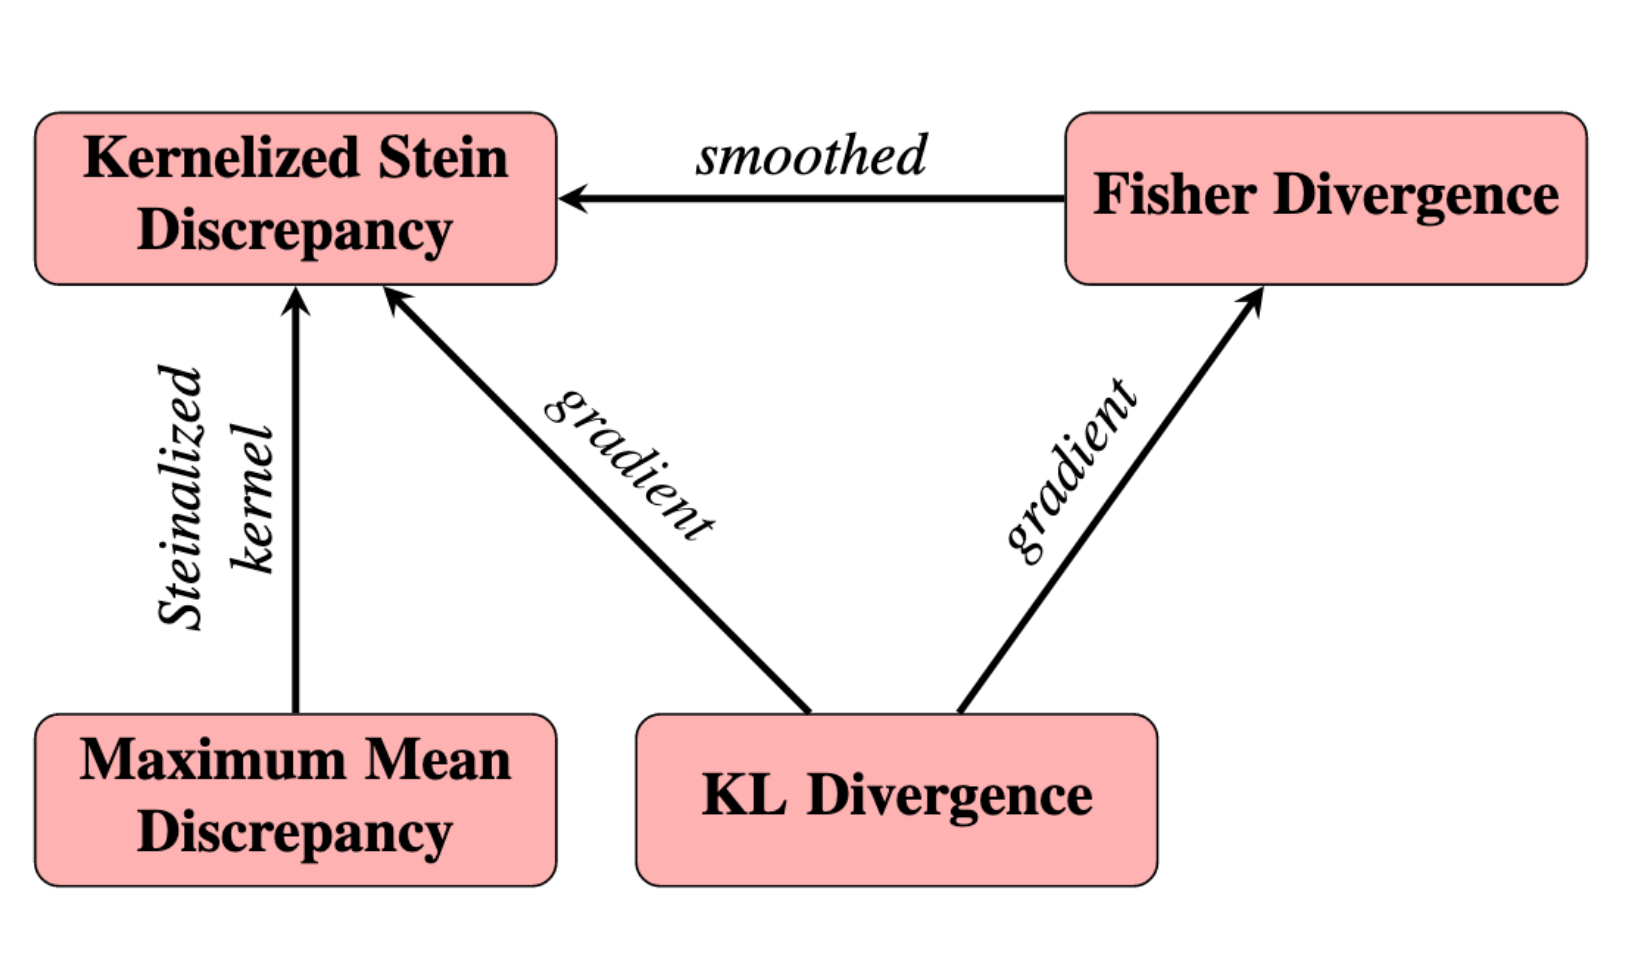
\includegraphics[width=.7\textwidth]{fd_ksd_mmd_kl.png} %
    \end{center}
    \label{fig:link-divergences}
    \caption{Relationships between the Fisher Divergence, the KL divergence, the MMD, and the KSD \cite{liu2016short}}
\end{figure}

\section{Experimental Results}

This section contains visualizations of all experiments discussed in \cref{main-sec:experiments}, including figures contained in the main text.
In all experiments we set the significance level to $\alpha = 0.05$.
Every experiment is repeated for 100 randomly sampled datasets and with 500 bootstrap iterations for estimating the quantile of the test statistic.

We use Gaussian distributions and compare the KCCSD and the SKCE with different combinations of kernels.
For the KCCSD, for Gaussian distributions all considered test statistics can be evaluated exactly.
Alternatively, for the exponentiated (kernelized) Fisher kernel and the exponentiated MMD kernel one can resort to approximations using samples from the base measure.
For the SKCE, however, the test statistic can be evaluated exactly on in special cases such as Gaussian kernels on the target space.
All approximate evaluations are performed with 10 samples.

\subsection{False Rejection Rate}

In this section we list the empirical false rejection rates for two calibrated datasets.

\subsubsection{Mean Gaussian Model}

\begin{figure}[!htb]
    \centering
    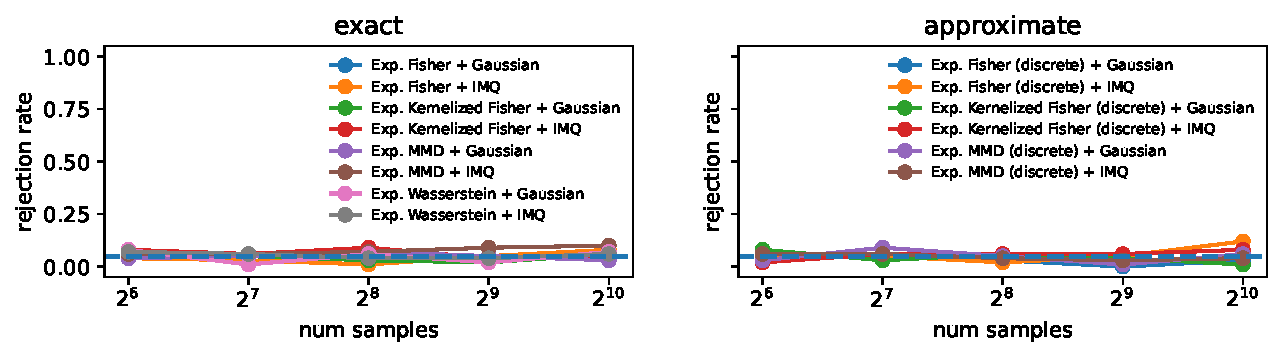
\includegraphics[width=\linewidth]{paper/figures/mgm_kccsd.pdf}
    \caption{False rejection rate of the KCCSD for MGM.}
\end{figure}

\begin{figure}[!htb]
    \centering
    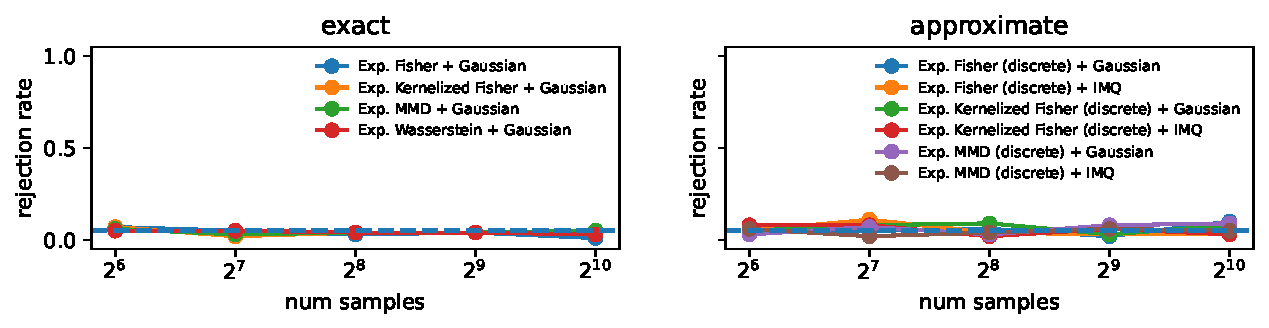
\includegraphics[width=\linewidth]{paper/figures/mgm_skce.pdf}
    \caption{False rejection rate of the SKCE for MGM.}
    \label{fig:mgm_skce}
\end{figure}

\subsubsection{Linear Gaussian Model}

\begin{figure}[!htb]
    \centering
    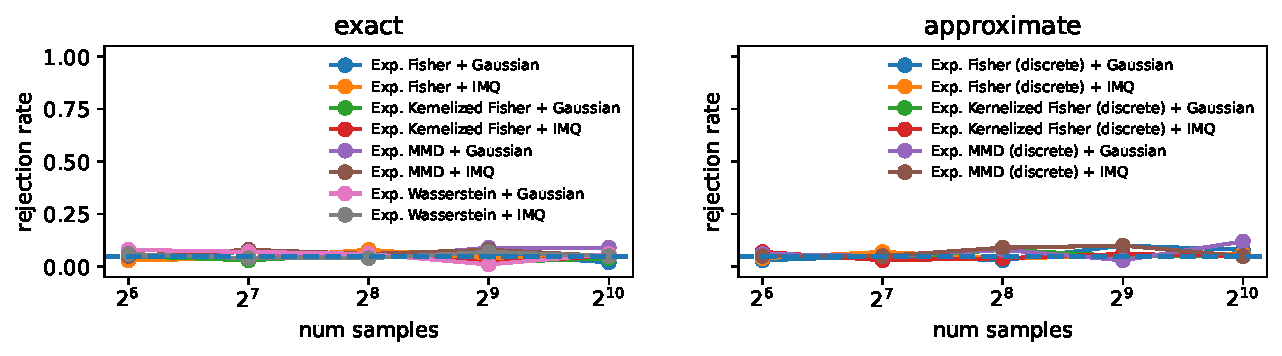
\includegraphics[width=\linewidth]{paper/figures/lgm_kccsd.pdf}
    \caption{False rejection rate of the KCCSD for LGM.}
    \label{fig:lgm_kccsd}
\end{figure}

\begin{figure}[!htb]
    \centering
    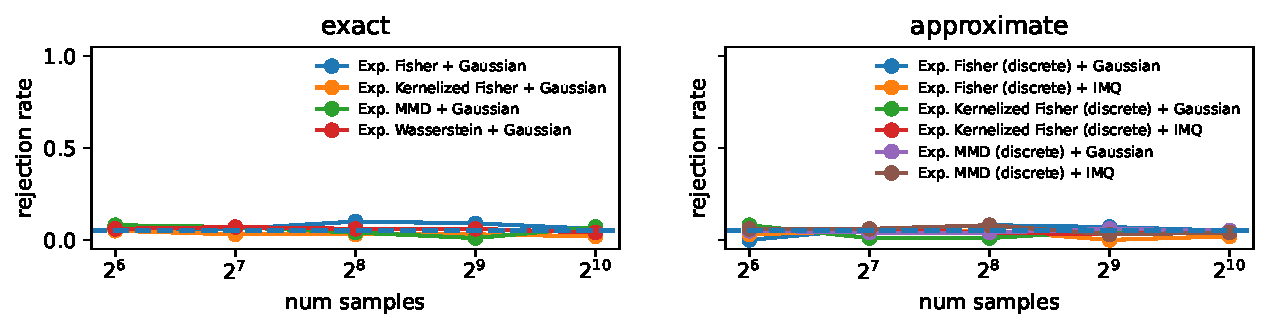
\includegraphics[width=\linewidth]{paper/figures/lgm_skce.pdf}
    \caption{False rejection rate of the SKCE for LGM.}
    \label{fig:lg_skce}
\end{figure}

\subsection{Test Power}

\subsubsection{Miscalibrated Mean Gaussian Model}

\begin{figure}[!htb]
    \centering
    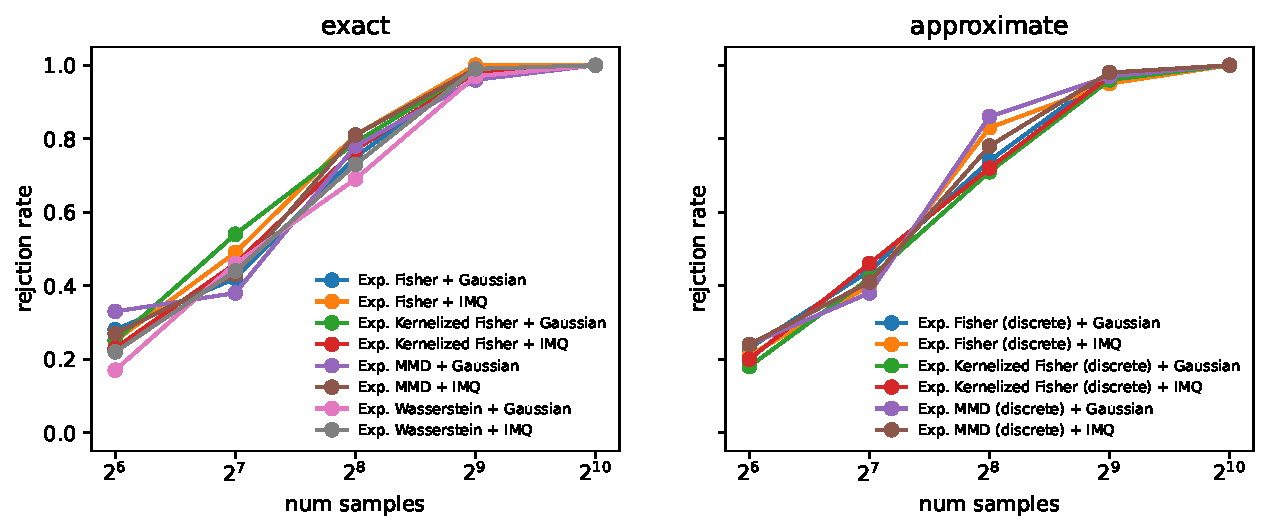
\includegraphics[width=\linewidth]{paper/figures/pmgm_kccsd_delta=0.1_shift-dim=-1.pdf}
    \caption{Rejection rate of the KCCSD for MMGM ($\delta = 0.1 \mathbf{1}_d$).}
    \label{fig:pmgm_kccsd_all}
\end{figure}

\begin{figure}[!htb]
    \centering
    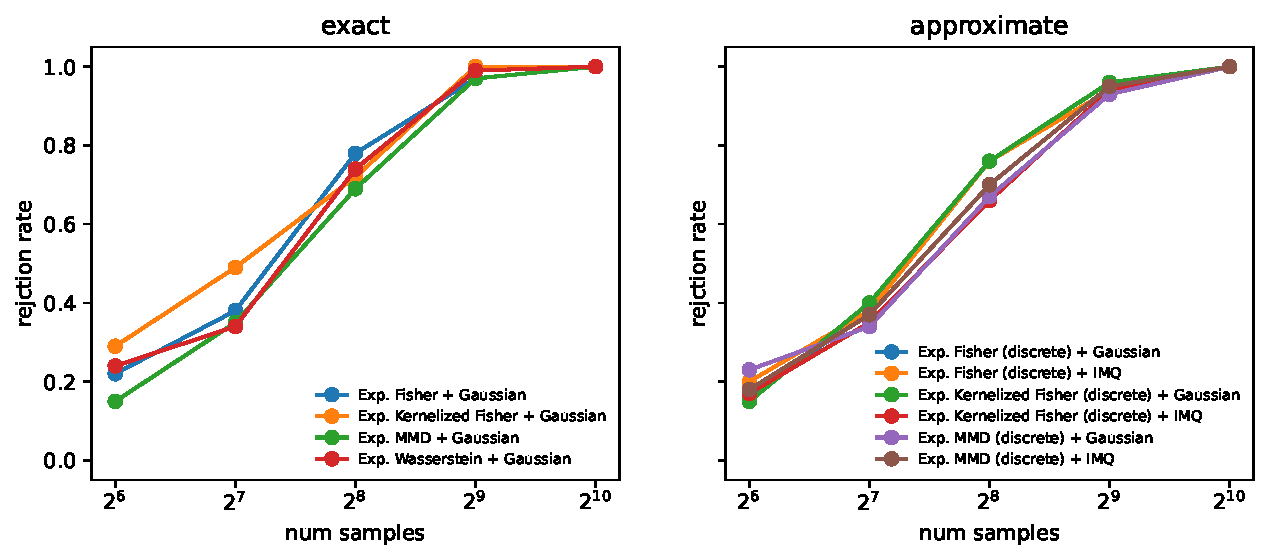
\includegraphics[width=\linewidth]{paper/figures/pmgm_skce_delta=0.1_shift-dim=-1.pdf}
    \caption{Rejection rate of the SKCE for MMGM ($\delta = 0.1 \mathbf{1}_d$).}
    \label{fig:pmgm_skce_all}
\end{figure}

\begin{figure}[!htb]
    \centering
    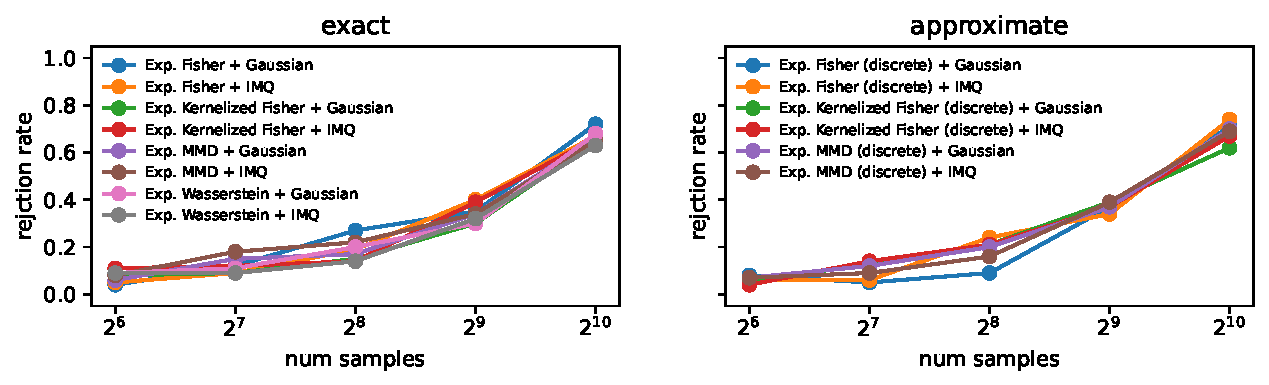
\includegraphics[width=\linewidth]{paper/figures/pmgm_kccsd_delta=0.1_shift-dim=1.pdf}
    \caption{Rejection rate of the KCCSD for MMGM ($\delta = 0.1 e_1$).}
\end{figure}

\begin{figure}[!htb]
    \centering
    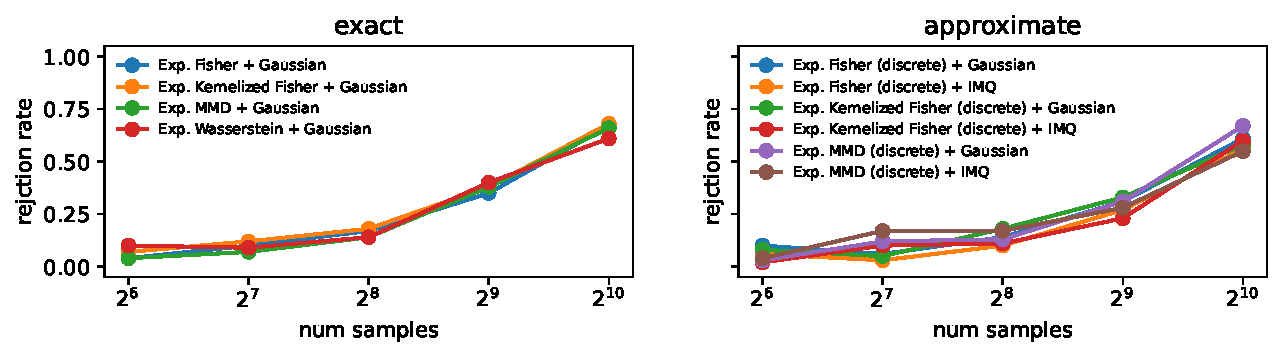
\includegraphics[width=\linewidth]{paper/figures/pmgm_skce_delta=0.1_shift-dim=1.pdf}
    \caption{Rejection rate of the SKCE for MMGM ($\delta = 0.1 e_1$).}
    \label{fig:pmgm_skce_first}
\end{figure}

\subsubsection{Heteroscedastic Gaussian Model}

\begin{figure}[!htb]
    \centering
    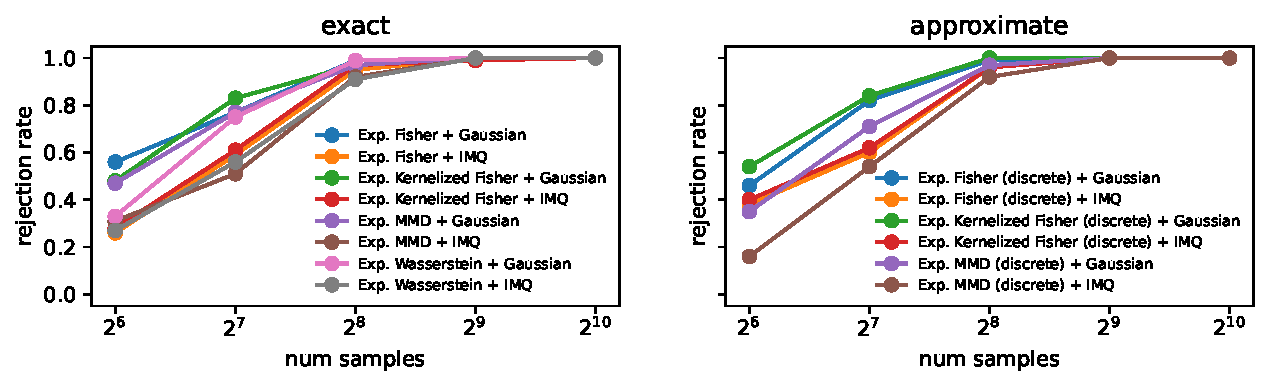
\includegraphics[width=\linewidth]{paper/figures/hgm_kccsd.pdf}
    \caption{Rejection rate of the KCCSD for HGM.}
    \label{fig:hgm_kccsd}
\end{figure}

\begin{figure}[!htb]
    \centering
    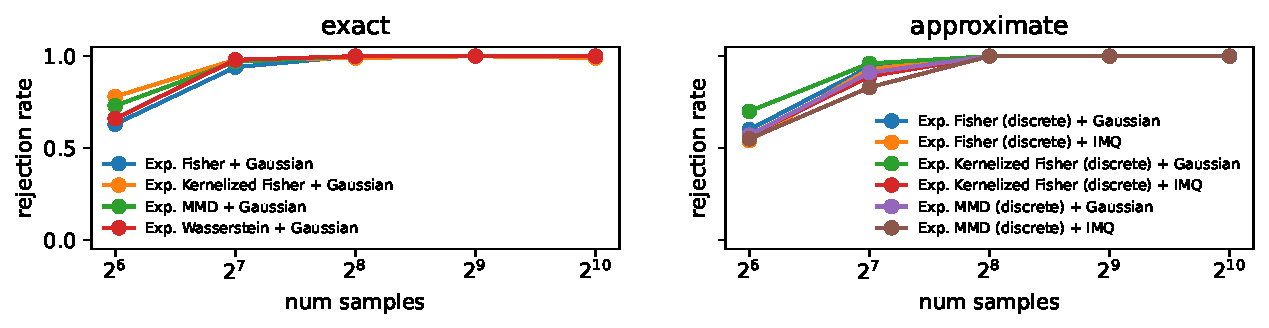
\includegraphics[width=\linewidth]{paper/figures/hgm_skce.pdf}
    \caption{Rejection rate of the SKCE for HGM.}
    \label{fig:hgm_skce}
\end{figure}

\subsubsection{Quadratic Gaussian Model}

\begin{figure}[!htb]
    \centering
    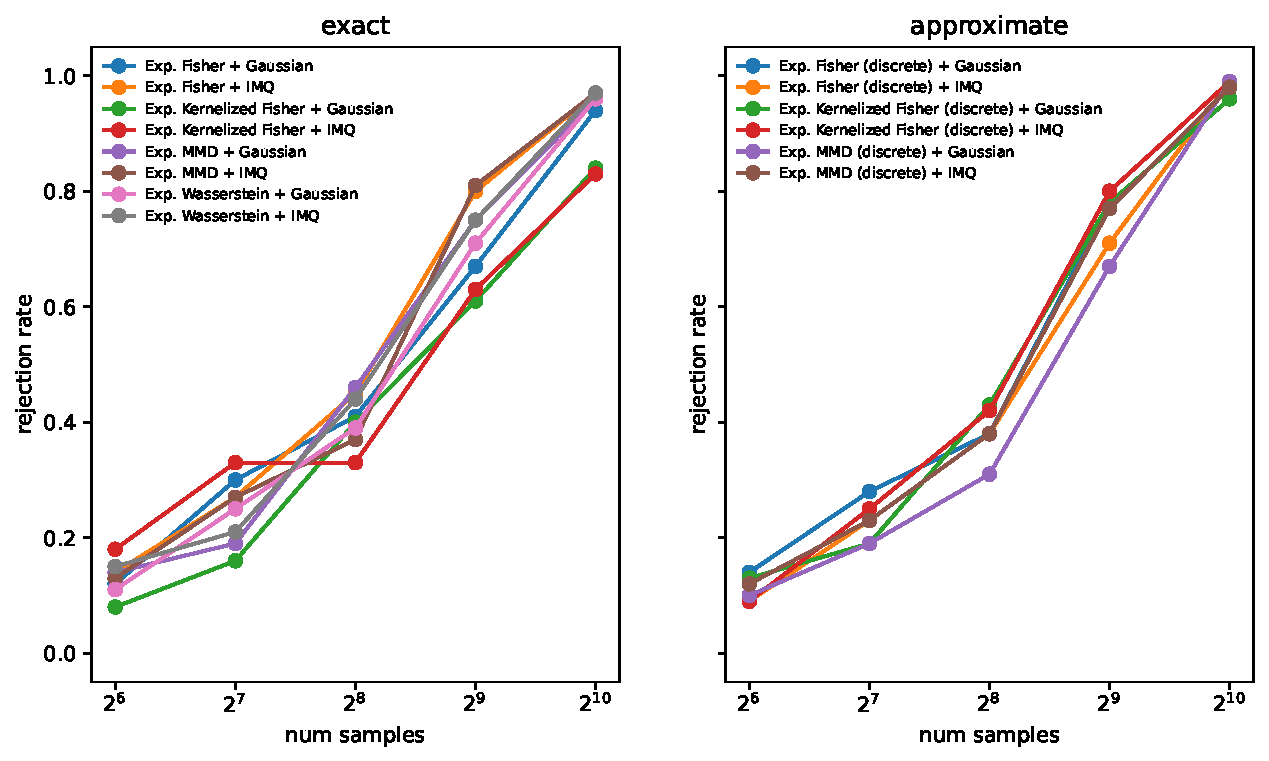
\includegraphics[width=\linewidth]{paper/figures/qgm_kccsd.pdf}
    \caption{Rejection rate of the KCCSD for QGM.}
    \label{fig:qgm_kccsd}
\end{figure}

\begin{figure}[!htb]
    \centering
    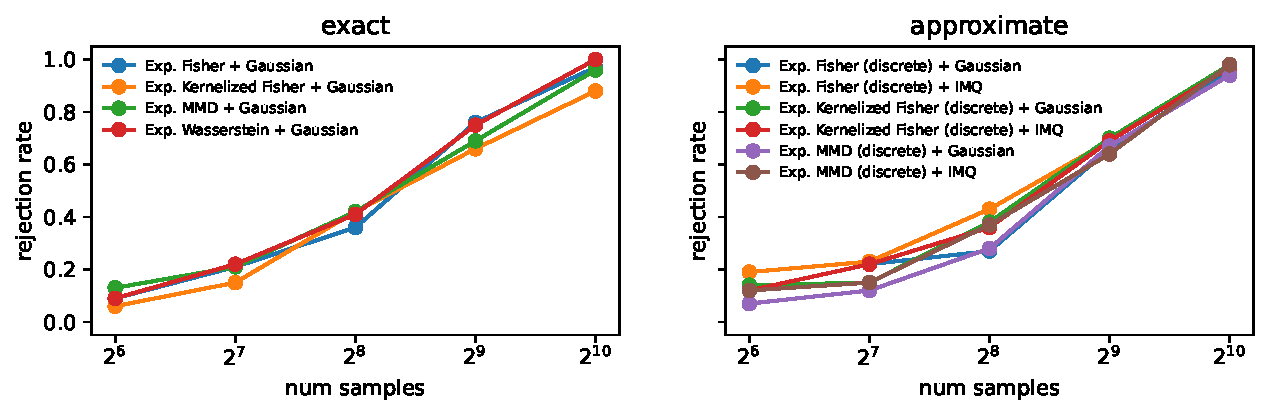
\includegraphics[width=\linewidth]{paper/figures/qgm_skce.pdf}
    \caption{Rejection rate of the SKCE for QGM.}
    \label{fig:qgm_skce}
\end{figure}

\bibliography{refs}

\end{document}
